\documentclass{sig-alternate}
\usepackage{tabularx}
\usepackage[noabbrev]{cleveref}
\usepackage{paralist}
\usepackage[table]{xcolor}
\usepackage[hidelinks]{hyperref}
%tiny urls
\makeatletter
\def\url@georgiostyle{%
  \@ifundefined{selectfont}{\def\UrlFont{\sf}}{\def\UrlFont{\scriptsize\ttfamily}}}
\makeatother

\urlstyle{georgio}

\begin{document}

% Copyright
\setcopyright{acmcopyright}
%\setcopyright{acmlicensed}
%\setcopyright{rightsretained}
%\setcopyright{usgov}
%\setcopyright{usgovmixed}
%\setcopyright{cagov}
%\setcopyright{cagovmixed}


% DOI
%\doi{10.475/123_4}

% ISBN
%\isbn{123-4567-24-567/08/06}

%Conference
%\conferenceinfo{PLDI '13}{June 16--19, 2013, Seattle, WA, USA}

%\acmPrice{\$15.00}

%
% --- Author Metadata here ---
\conferenceinfo{MSR}{'16 Austin, Texas USA}
% --- End of Author Metadata ---

\title{The Evolution of GHTorrent: Growing an Open Access Dataset 10x}
\numberofauthors{1} %  in this sample file, there are a *total*
% of EIGHT authors. SIX appear on the 'first-page' (for formatting
% reasons) and the remaining two appear in the \additionalauthors section.
%
\author{
% The command \alignauthor (no curly braces needed) should
% precede each author name, affiliation/snail-mail address and
% e-mail address. Additionally, tag each line of
% affiliation/address with \affaddr, and tag the
% e-mail address with \email.
%
% 1st. author
\alignauthor Georgios Gousios\\
       \affaddr{Radboud University Nijmegen}\\
       \affaddr{Nijmegen, the Netherlands}\\
       \email{g.gousios@cs.ru.nl}
}

\maketitle
\begin{abstract}

With over 31 million repositories and 12 million users, GitHub is by far the
biggest open source forge in existence. Since early 2012, the GHTorrent project
has been retrieving data from GitHub's open access {\sc api} and offering them
to the repository mining community. In this paper, we describe how we grew
GHTorrent to ten times the size of early 2013, while at the same time improving
its coverage, quality, and versatility and offering free and open data access
services to hundreds of researchers.

\end{abstract}

%
% The code below should be generated by the tool at
% http://dl.acm.org/ccs.cfm
% Please copy and paste the code instead of the example below. 
%
\begin{CCSXML}
<ccs2012>
<concept>
<concept_id>10010405.10010476.10003392</concept_id>
<concept_desc>Applied computing~Digital libraries and archives</concept_desc>
<concept_significance>500</concept_significance>
</concept>
<concept>
<concept_id>10002951.10003227.10003351</concept_id>
<concept_desc>Information systems~Data mining</concept_desc>
<concept_significance>300</concept_significance>
</concept>
<concept>
<concept_id>10003120.10003130.10003233.10003597</concept_id>
<concept_desc>Human-centered computing~Open source software</concept_desc>
<concept_significance>300</concept_significance>
</concept>
</ccs2012>
\end{CCSXML}

\ccsdesc[500]{Applied computing~Digital libraries and archives}
\ccsdesc[300]{Information systems~Data mining}
\ccsdesc[300]{Human-centered computing~Open source software}

%
%  Use this command to print the description
%
\printccsdesc

\keywords{Dataset, GitHub, GHTorrent}

\section{Introduction}

GHTorrent was first presented as a proof-of-concept in 2012~\cite{GS12} and as a
complete version in 2013~\cite{Gousi13}. Since then, it has been one of the most
popular datasets for the repository mining community. Apart from traditional
repository mining, it has been frequented as an easy-to-use initial filter
before repository analysis, as a data mining competition
dataset,\footnote{\url{https://github.com/blog/1864-third-annual-github-data-challenge}}
as educational
material,\footnote{e.g. \url{http://web.stanford.edu/class/cs224w/resources.html}}
as and as a basis for other tools.  By itself or through
derivative work, it has been featured several times on popular developer news
sites.\footnote{e.g. \url{https://news.ycombinator.com/item?id=8818035} and\\
\url{https://redd.it/2ig8yz}}

GitHub is a lively community of collaborating developers; since GHTorrent
started, its user base grew from 1.2 million users to 12 million users and the
number of hosted repositories from 4 million to 30 million. GitHub's users are not idle,
either; as Figure~\ref{fig:growth} shows, the number of events triggered by user
actions has been growing exponentially. GHTorrent attempted (as
Table~\ref{tab:stats} shows) to keep up with the increased traffic using two
strategies: i) extensive profiling and optimization of both GHTorrent's code
base and the underlying services and ii) relying on its user community for
GitHub {\sc api} keys.

In this paper, we outline the progress of GHTorrent since 2013; we focus on the
steady improvements and adaptions to GHTorrent and the way it provides users
access to its datasets. We skip a generic introduction to GHTorrent itself, for
which we refer interested readers to references~\cite{GS12} and~\cite{Gousi13}.
We complement this work with a list of (still) open and promising research
topics that can be explored using GHTorrent.

\section{New developments}

Changes to the data {\sc api} endpoints at GitHub and issues in the data
collection process, as well as responding to user requests, led to a series of
improvements in GHTorrent. We present the most important ones below.

\begin{table}
  \centering
  \begin{small}
    \label{tab:datasetsize}
       \resizebox{0.95\linewidth}{!}{
  \begin{tabular}{llll}
    \hline
    \bfseries{Entity} & \bfseries{MongoDB} & \bfseries{MySQL} & \bfseries{$\Delta_{2016/2013}$} \\
    \hline
\rowcolor[gray]{0.95}      Events                     & 476,047,453 & ---           & 11.1x\\
      Users                      & 6,733,244   & 9,277,113     & 8.4x \\
      \ldots of which fake       & ---         & 2,435,859     & ---\\
      \ldots of which deleted    & ---         & 271,590       & ---\\
      \ldots of which geolocated & ---         & 1,108,784     & \\
\rowcolor[gray]{0.95}      Repositories               & 28,851,321  & 25,578,419    & 21.8x\\
\rowcolor[gray]{0.95}      \ldots of which forks      & ---         & 10,486,114    & --- \\
\rowcolor[gray]{0.95}      \ldots of which deleted    & ---         & 4,986,095     & ---\\
      Commits                    & 367,815,284 & 362,057,838   & 12.3x \\
\rowcolor[gray]{0.95}      Issues                     & 24,165,582  & 25,351,996    & 10.3x \\
      Pull requests              & 11,944,969  & 11,114,625    & 9.7x \\
\rowcolor[gray]{0.95}      Issue comments             & 42,021,374  & 43,416,372    & 14.6x\\
      Watchers (stars)           & 51,698,373  & 37,022,681    & 6.6x\\
      \hline
  \end{tabular}
  }

%    \begin{tabular}{llll}
%      \hline
%      \multicolumn{3}{l}{\bfseries{Service statistics}}\\
%      \hline
%      Programmatic access users  & 150         &&\\
%      \ldots of which per day    & 1-2         &&\\
%      GitHub {\sc api} keys            & 55          &&\\
%      Monthly web users          & 2000        &&\\
%      \hline
%  \end{tabular}
    \caption{GHTorrent database contents on Jan. 14, 2016. The difference column reports the difference to 2013~\cite{Gousi13}.}
  \end{small}
  \label{tab:stats}
\end{table}

\subsection{Three operation modes}

GHTorrent follows GitHub's event stream and retrieves the linked entities using
a dependency-based recursive retrieval process. For example, whenever a
developer pushes (possibly several) commits to GitHub, GitHub creates a nested
PushEvent on the event stream, comprising information such as the transferred
commits, their contents, and target repository. GHTorrent picks up the events on
the stream and then it retrieves all commits, committers and repositories that
are linked through the PushEvent.

Through the years, we discovered that this mode of operation, while efficient,
has three issues: i) in case of the frequent failures (see
Figure~\ref{fig:service-stats}), the resulting data is inconsistent,
ii) we cannot update volatile information about users and projects (e.g. user
locations) as GitHub does not emit any related events, and
iii) we cannot collect all data for projects that existed before GHTorrent.
For these reasons, we introduced two additional operating modes:

\begin{compactdesc}

  \item[Full-repo / user retrievals.] When an error is reported by a GHTorrent
    user for a specific repository or a collection of repositories, we run a
    process that retrieves all information about a given user or repository
    recursively. The same process has been used by several Open Source Software
    ({\sc oss}) projects to generate community analytics; the
    GHTorrent-Vagrant\footnote{\url{https://github.com/ghtorrent/ghtorrent-vagrant}}
    project was thus created to streamline the installation of GHTorrent for
    such projects.

  \item[Bi-monthly update.] For each non-deleted repository and user in the
    database, GHTorrent retrieves a fresh copy of its entry on GitHub. This way,
    GHTorrent can mark projects and users as deleted (they exist in GHTorrent
    but not on GitHub) or update their metadata (e.g. programming
    languages).

\end{compactdesc}

Furthermore, to eliminate data retrieval holes caused by arbitrary errors in
collecting the event stream, we synchronize the contents of the event collection
with GitHub Archive\footnote{\url{https://www.githubarchive.org}} daily.

\begin{figure}
  \begin{center}
    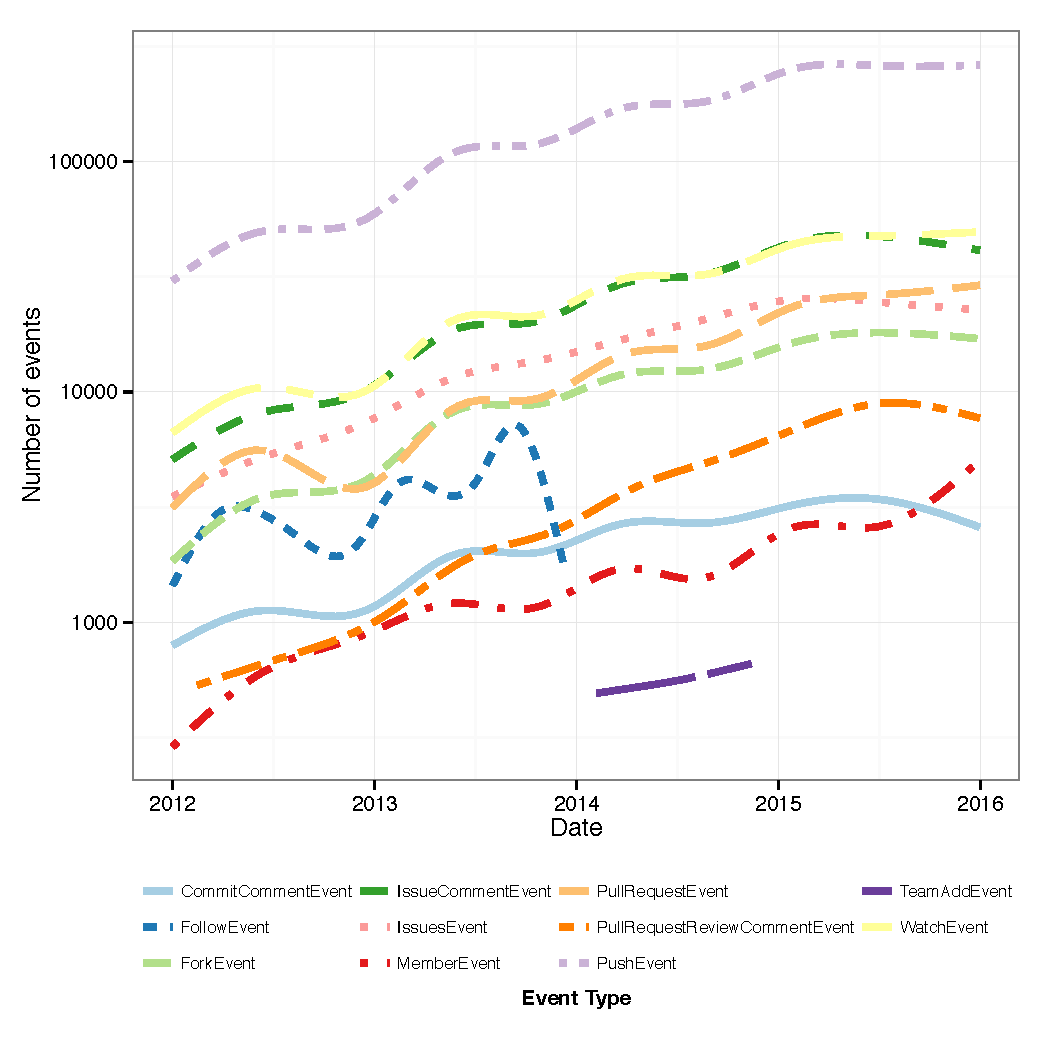
\includegraphics[scale=0.5]{github-growth}
  \end{center}
  \vspace{-1em}
  \caption{Number of events per type generated per day (smoothing has been
  applied).}
  \vspace{-1em}
  \label{fig:growth}
\end{figure}

\begin{figure}
  \begin{center}
    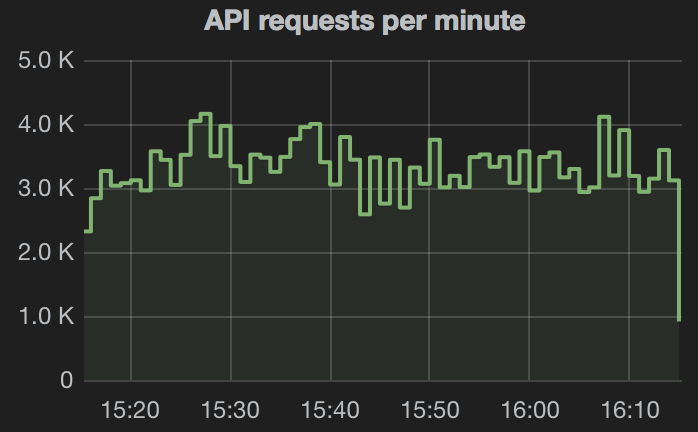
\includegraphics[scale=0.332]{api-requests}
    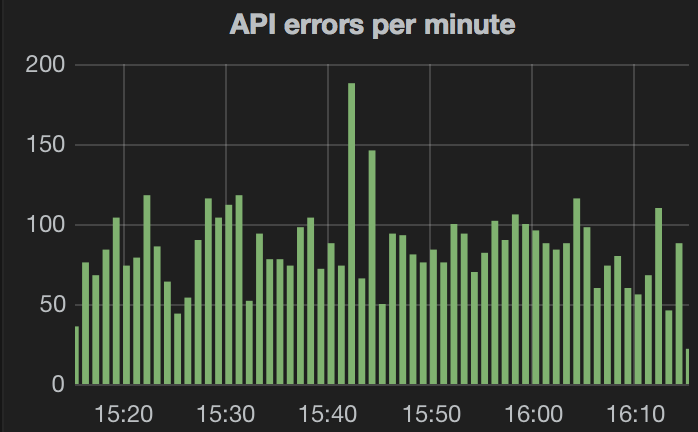
\includegraphics[scale=0.332]{api-errors}
    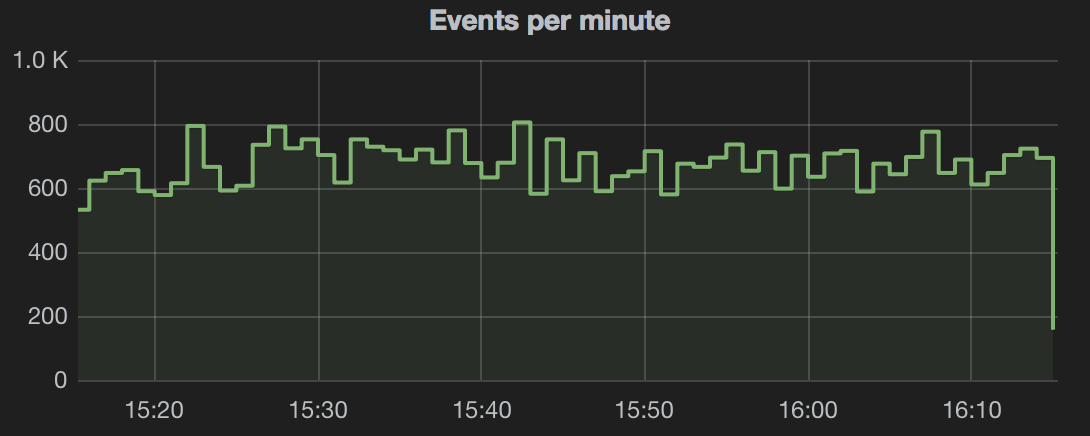
\includegraphics[scale=0.438]{events-per-min}
  \end{center}
  \vspace{-1em}
  \caption{Service monitoring graphs for a typical day (Jan 18,
  2016).}
  \vspace{-1em}
  \label{fig:service-stats}
\end{figure}

\subsection{Repository Languages}
GitHub calculates programming language usage statistics for a
repository by default. Upon visiting its main page on GitHub, the user sees this
information as horizontal bar:

\noindent
\includegraphics[scale=0.243]{languages}

Until February 2015, this information was not available through the {\sc api}
and researchers could thus only rely on the main repository language when
selecting repositories for analysis. This led to sub-optimal repository
selections. As of November 2015, GHTorrent collects fine-grained size
information (in bytes) for all programming languages in all repositories; this
information is time-stamped with the retrieval date. With it,
researchers can refine the selection of repositories, cluster repositories in
new ways (e.g. those that contain Javascript and HTML are probably web
projects), and even analyze the evolution of programming language use.

\subsection{Forks}

When a project is forked, GitHub will create an identical copy of the project
repository and initialize a new issue tracker for it. Internally, the repository
contents are not really duplicated; GitHub will use a copy-on-write mechanism to
minimize disk space
use.\footnote{\url{http://githubengineering.com/counting-objects/}} When GHTorrent
encounters a fork event, it has to treat the fork as a new repository. This
process makes forking very cheap for GitHub, but very expensive for GHTorrent.

GHTorrent recursively retrieves all information about the fork, such as the
repository owner and issue labels. In early versions, recursive
retrieval also included commits. For big and popular projects, such as Ruby on
Rails (55k commits, 11k forks), this process required several (thousand)
additional GitHub {\sc api} calls, which quickly depleted GHTorrent limited {\sc
api} rates. For this reason, GHTorrent implemented a mechanism that only
retrieves new commits from forks until it finds a shared commit with the parent
repository; it would then switch to copying commits internally within the
GHTorrent database. This trick worked with formidable efficiency, as it cut down
on {\sc api} calls (and the time required to process them) by more than 95\% for
big projects.

However, its very efficiency caused a new problem; \emph{too many} processed
forks meant that the table that records the association between commits and
repositories (\texttt{project\_\-commits}) grew uncontrollably. Just for Ruby
on Rails, this table would store more than 500M rows. The root of the problem
is that \texttt{project\_commits} models an $M \times N$ relationship between
projects and commits and this cannot be normalized further without significant
duplication (Boyce-Codd normal form).

Consequently, retrieving fork commits was converted to an optional
configuration parameter and not retrieved by default. Therefore, the
(\texttt{project\_\-commits}) table is inconsistent with respect to
fork commits.

\subsection{User and Repository Descriptions}

When a commit is processed by GHTorrent, a user must be associated with it.
GHTorrent first attempts to query GitHub for information about the committer
and, if this fails (the committer is not registered with GitHub), then it
creates a fake user to register this commit with. Until recently, it was not
possible to identify fake users; GHTorrent now marks them as such in the MySQL
database. Moreover, it can retroactively convert fake users to normal users if
a user with the provided email is registered with GitHub in the future.

Users can also delete their accounts. GHTorrent keeps track of deleted users by
marking them. This helps researchers to eliminate inactive users from
their analyses.

Similarly to users, repositories are marked as deleted if GHTorrent cannot find
them during the bi-monthly update cycle anymore. To inform researchers about
the last full repository update, the projects table includes an
\texttt{updated\_at} field. Finally, the \texttt{forks} table has been removed
and the parent repository information is being kept more conveniently in the
\texttt{forked\_\-from} field of the repository entry itself.

\subsection{User Geolocation}

Almost 1.3M GitHub users share their location in their profiles. GHTorrent uses
this information to \emph{geolocate} those users. Geolocation refers to the
process of converting a text string potentially indicating the address of a
place on earth to the longitude and latitude co-ordinates corresponding to this
address. As GitHub's address field is free-form text, there are no guarantees
about the format of the address fields. GHTorrent uses the OpenStreetMap
geolocation service (Nominatim) for this functionality. To overcome Nomitatim's
{\sc api} restrictions, it caches geolocated places in the Mongo
database. 160,000 cached addresses have been collected so far, with a very high
cache hit ratio.  An example application of geolocation information can be seen
in Figure~\ref{fig:dev-map}.

It is important to notice that geolocation in GHTorrent is a best effort
approach. Initially, not all user provided location strings can be decoded to a
real address; on the one hand, several users provide fictional addresses.  On
the other hand, users may choose not to share their addresses due to cultural
differences in online privacy perceptions, possibly leading to user clusters in
certain regions being under-represented. Consequently, care must be applied
when drawing conclusions from this data.

\begin{figure}
  \begin{center}
    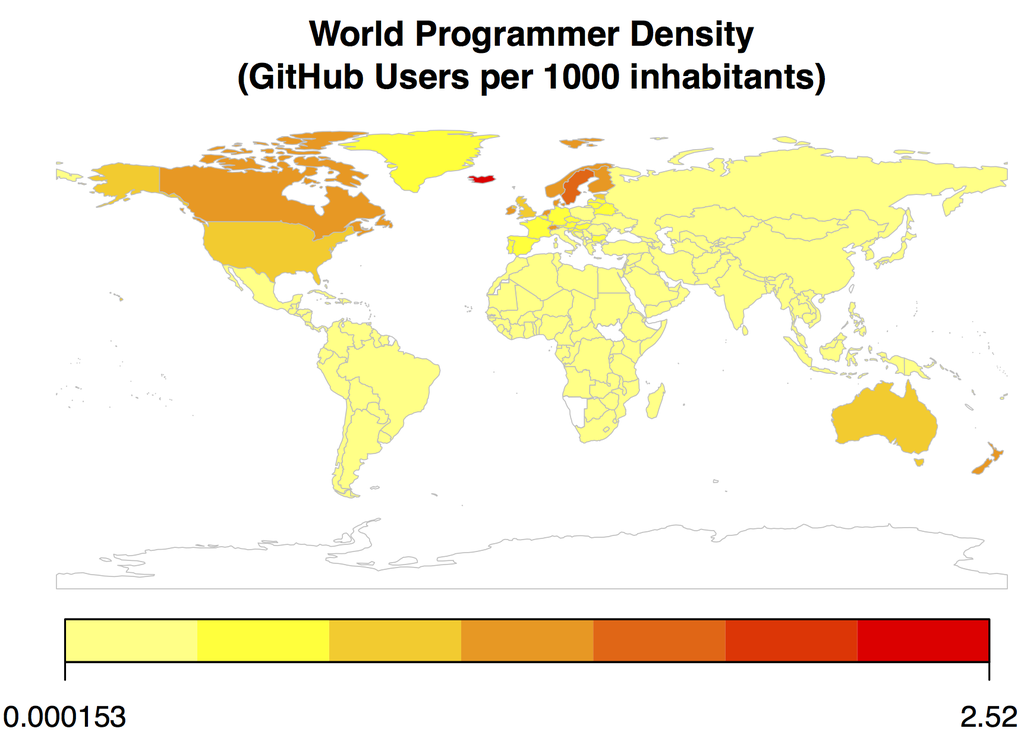
\includegraphics[scale=0.2]{dev-map.png}
  \end{center}
  \vspace{-1em}
  \caption{GHTorrent users that registered a location plotted on a map after
  geocoding them.}
  \label{fig:dev-map}
  \vspace{-1em}
\end{figure}

\subsection{Discontinued and Incomplete}

The following services or features have been discontinued:

\begin{compactdesc}

  \item[Repository Collaborators and Organization Members] On Nov 2014, GitHub
    disabled the repository membership query endpoint. It is therefore
    impossible to determine which users have commit access to the repository in
    a straightforward manner. Interestingly, they did not completely hide this
    information; when a user is added as a member, a MemberEvent is fired. As
    GHTorrent follows the event stream, it can retrieve new repository members,
    but it cannot update membership information during the bi-monthly update
    cycles. Moreover, GitHub made the organization membership information
    private to organizations by default (with the option of making it public
    resting with the organization), which does not allow GHTorrent to update
    organization members from all organizations.

  \item[Followers] GitHub does not emit follow events since late 2013. However,
    the {\sc api} endpoint does permit to retrieve user followers, so GHTorrent
    collects followers during the bi-monthly user update cycle. However, the
    timestamp of the follow action cannot be recorded accurately.

  \item[Lean GHTorrent] Lean GHTorrent~\cite{GVSZ14} was effectively a dataset
    slicer for GHTorrent users that could not use the dataset in its
    entirety. In two years of operation, Lean GHTorrent only received 55 user
    requests. To the best of our knowledge, no visible work resulted from its
    use. As of January 2016, Lean GHTorrent is discontinued.

\end{compactdesc}

\subsection{Azure and Data Lake}
GHTorrent's data collection process was recently moved to the Azure cloud
platform. The move to Azure was important for two reasons: i) to ensure the
sustainability of GHTorrent in the face of growing hardware requirements ii) to
better allocate available developer resources to the future of GHTorrent. The
move was motivated by a donation of free Azure usage credits.

The move to Azure has the following benefits for the research community:

\begin{compactitem}

  \item GHTorrent servers are now more capable of dealing with the accumulated
    data sizes and GitHub growth. This means more accurate data collection
    and more frequent retrospective updates.

  \item The online dataset access services will run on more powerful servers,
    leading to better query performance and access to real-time replicas of
    the main project databases.

  \item The dataset and collection process will be integrated with Azure
    Data Lake, a big data processing platform featuring a common backend
    and multiple front ends. Researchers will be soon able to use state
    of the art big data analysis tools (e.g. {\sc usql}, Spark) to scale
    research across all GHTorrent data in real-time.

\end{compactitem}


\subsection{Service updates}

The following changes took place in the way the GHTorrent data collection
and distribution is being run:

\begin{compactdesc}

  \item[Backups] GHTorrent distributes bi-weekly MySQL dumps and daily MongoDB
    backups.

  \item[Programmatic access] GHTorrent offered programmatic access over
    {\sc ssh} tunnels to MongoDB since late 2013. Programmatic access to the
    live MySQL server is planned for the second quarter in 2016.

  \item[GitHub {\sc api} keys] In exchange for programmatic access, GHTorrent
    asks interested parties to (voluntarily) provide GitHub {\sc api} keys. We
    have currently collected 50 active {\sc api} keys, which enabled us to run
    the bi-montly update cycle.

\end{compactdesc}

%\section{Lessons learned}



\section{Open research topics}
GHTorrent has been in the center of several research
efforts; we estimate that close to 60 papers have been written using data from
GHTorrent.\footnote{GHTorrent's ``Hall of fame'' page lists at least 20:\\
\url{http://ghtorrent.org/halloffame.html}} With GHTorrent data, schemata and
limitations being understood by a large number of software engineering
researchers, new capabilities on offer and a large scale data analysis
infrastructure in place, the research community can collaborate to answer deeper
questions and impact the daily practice of millions of developers.

Below, we present a collection of open research topics that can be answered
with large-scale quantitative or mixed-method studies using GHTorrent.

\noindent{\bfseries Developers.} Not all GitHub users are software developers;
web designers, testers, amateur programmers. and students use GitHub to
collaborate in open projects. Different users have different needs and
contribute in different capacities to {\sc oss}; to provide customized support
to them, it is important to devise algorithms to cluster them in groups based on
their activity traces. Research in clustering methods can investigate signals
such as the technology stack used, interaction types, physical location and
contribution networks. On the same note, it is important to investigate how
\emph{communities} of similar GitHub users work together to build large {\sc
oss} projects. Finally, the extraction of developer profiles, for example
comprising programming languages, domain expertise, and contribution types can
facilitate the automated assignment of developers to incoming issues or the
matching of developers to job descriptions.

\noindent{\bfseries Projects.} A common issue faced by researchers when analyzing
repositories on GitHub is the automated determination of the kind of contents a
repository hosts. This issue is complicated by the fact that most repositories
are small and inactive~\cite{KGBSGD15}, while, as Table~\ref{tab:stats}
presents, almost half of them are forks. We need methods to classify
repositories into types based on source code or other artifacts (e.g. libraries,
front end frameworks, web interfaces etc).  Furthermore, it is helpful to
determine the application domain (e.g. web development, financial analysis,
scientific software etc) that a repository is a part of, as this will enable
cross-domain studies of development methods and styles.

\noindent{\bfseries Software Ecosystems} Much of the open source development,
especially in areas such as software tools and libraries for web development, is
taking place on GitHub. The use of standardized software library management
tools (e.g. \textsf{npm} for Javascript or \textsf{gem} for Ruby) along with the
centralized hosting allows researchers to examine the full dependency graph
among libraries and their users at the method call level. Researchers can then
examine issues such as propagation of security flaws, clustering of programming
languages in various application domains and develop methodologies for
data-driven {\sc api} evolution.

\noindent{\bfseries Community best practices} Existing research on \textsf{oss}
development has identified several patterns of collaborative development (e.g.
the onion model~\cite{Yunwe03}). This research however assumed community
organizations very different than what GitHub affords; the ability to submit a
pull request to any project on GitHub effectively flattens the organizational
hierarchy and makes the contribution process more streamlined. New research
should identify the emerging community structures and learn the dynamics behind
their evolution. Related is the topic of community effectiveness; it is
important to understand what makes communities effective in attracting and
maintaining contributors, and extract best practices to help future communities
evolve. Which teams and projects are more productive and what are their
practices and patterns?

\noindent{\bfseries Trends and outliers} One might argue that the majority of
{\sc oss} development is being done on GitHub; even projects that are not
GitHub-based, often have a mirror on GitHub. This gives researchers a tremendous
opportunity to do almost full population studies to identify software technology
trends, such as architecture patterns, popularity of programming languages and
tools. Moreover, it may be interesting to identify corner cases and technology
outliers; what are the factors and processes that make certain projects, such
as \textsf{node.js} and Ruby on Rails, instant successes? Longitudinal studies
can help in modeling the processes that make technologies more prone to
widespread adoption.

\section{Conclusions}

In this work, we presented the recent evolution of the GHTorrent dataset.
GHTorrent will continue to evolve along with GitHub and adapt to user
requirements in the foreseeable future.

The exploration of the wealth of data provided by GitHub has just begun to
scratch the surface. As a research community, we must scale our research
efforts, identify, target, and solve real world issues that affect one of the
most important fields of economic activity today: the collaborative production
of software.

\section*{Acknowledgements}

The GHTorrent project would like to thank Microsoft for their generous support
that enabled the move to the Azure cloud. The author would also like to thank
the numerous GHTorrent users (Bogdan Vasilescu and Daniel German require
special mention) for the fruitful discussions that led to a better GHTorrent
for everybody. Finally, the author would like to thank Trevor Carnahan for the
interesting discussion that led to the list of open research topics and
Moritz Beller for the best review ever.

\newpage

\bibliographystyle{acm}
\bibliography{ghtorrent-update}


\end{document}
